\chapter{Central de procesamiento}
\section{Descripción general}
\par El diseño general del sistema se pensó como tres nodos de escucha que son comandados
por medio de una central de procesamiento. Los requerimientos de la misma se
establecen para lograr una comunicación estable y segura con cada uno
de los nodos, donde en caso de detectar una inhibición por parte de cualquiera de ellos, requiera
el estado de los otros dos para así activar las alarmas correspondientes, comunicarse al
servidor web y volver a iniciar el sistema de cero una vez que se haya terminado el proceso
correctamente, dando también un reporte del estado de salud de cada nodo en particular.
\par En este capítulo se presentará la forma en que se llevó a cabo el desarrollo de la
misma, indicando su funcionamiento, primer prototipo, diseño final y la implementación de
un gabinete. 
\subsection{Funcionamiento}
\par El funcionamiento de la centrañ se podría dividir en tres partes interconectadas que se detallan a continuación.
\subsubsection{Comunicación con nodos}

\par Como ya se detalló en el apartado \ref{cap:max485}, la comunicación optada para la conexión de los 4 dispositivos es RS485 por su forma de transmisión diferencial y largo alcance. 
\par Al inicio del sistema la central (funcionando como el maestro en la comunicación) requiere el estado de cada nodo, del cual si alguno detecta una inhibición comenzaría el proceso para ver el estado de los demás nodos y comenzar a activar alarmas.

\subsubsection{Alarmas locales}
\par Una vez detectada la inhibición y procesado el estado del sistema en general se dan las alarmas visuales y sonoras en la central misma para dar aviso al personal de seguridad que se encuentra en el lugar. 

\subsubsection{Comunicación remota al servidor web}
\par Como ya vimos en el apartado \ref{cap:sim800l}, la comunicación con el servidor web se hace de manera remota mediante GPRS una vez que se encuentra el sistema en un estado de alarma, cargando en el mismo la ubicación, ID de nodos, entre otros que se detallarán en las siguientes secciones. 

\section{Prototipo}
\subsection{Diseño}
\subsubsection{PCB}
\par En la figura \ref{im:pcb-prototipo} podemos ver una vista superior (izquierda) e inferior (derecha) de la placa prototipo para llevar a cabo la implementación de esta. 
\begin{figure}[h!]
\begin{center}
    \subfigure{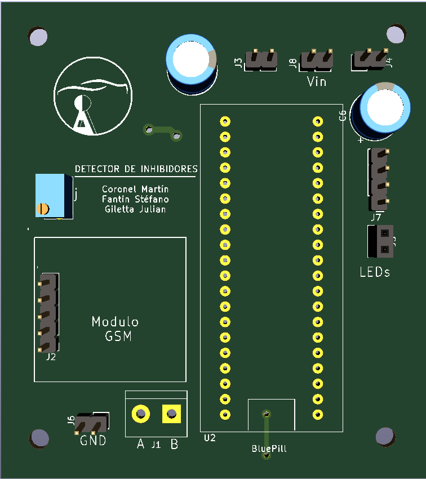
\includegraphics[width=60mm]{images/central/placa-prot-central-superior.png}}
    \subfigure{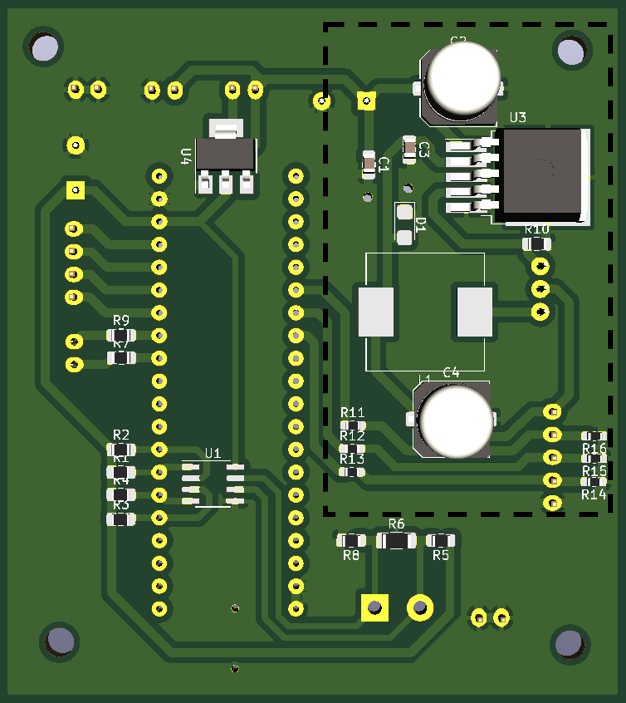
\includegraphics[width=60mm]{images/central/placa-prot-central-inferior.png}}
    \caption{Prototipo de placa de la central de procesamiento.}
	\label{im:pcb-prototipo}
\end{center}
\end{figure}

\subsection{Problemas surgidos}
\par Los principales problemas de esta primer aproximación al diseño final fueron en
base a la alimentación requerida por el integrado de comunicación GPRS.
\par En primer lugar, era necesario un capacitor en la alimentación del SIM800 para
suavizar el arranque del mismo, ya que al conectarse a una red GSM/GPRS requiere un pico
de corriente de 2A.
\par Por otra parte, al tener que rediseñar la placa, notamos que la fuente conmutada implementada (encerrada en lineas cortadas en la figura \ref{im:pcb-prototipo}) requería gran cantidad de componentes, aumentando así el costo, principalmente con el integrado e inductor necesarios. Por ello, se optó como solución un regulador lineal que con tan solo dos capacitores y dos resistencias se obtienen los requerimientos necesarios. 

\section{Diseño final}
\subsection{Software}
\par Para no volver redundante la explicación respecto del prototipo, se optó que el
funcionamiento del sistema embebido se detalle en esta sección ya que en cuanto a este no
fueron grandes los cambios realizados. 
\par En este apartado se nombraran como se llevaron a cabo los siguientes items:
\begin{itemize}
    \item Comunicación con nodos
    \item Salud de nodos
    \item Alarma sonora y visual
    \item Subida de datos al servidor web
\end{itemize}

\subsubsection{Comunicación con nodos}
\par Comenzamos nombrado esta etapa ya que es la tarea mas importante que ocurre en el dispositivo, un buen esquema de comunicación determina el buen funcionamiento del sistema en fin, ya que si bien los nodos son los encargados de detectar las inhibiciones, la central es el maestro que activa o no las alarmas y avisos. 
\par Como ya se nombró en la sección \ref{cap:max485}, la comunicación RS485 es half-duplex y debe existir un dispositivo maestro (en nuestro caso es el que se esta desarrollando), el cual es el encargado de generar requerimientos a cada dispositivo de la red y, si es necesario, esperar una respuesta de estos. 
\par Para entender el funcionamiento podemos ver la imagen \ref{im:maq-est-central} en donde se observan 3 columnas correspondientes cada una a un estado de funcionamiento.
\par En el estado 0, la comunicación es continua y rige un ciclo de un requerimiento de nodo por ves. La palabra es de 2 bytes, donde el primero corresponde al ID del nodo requerido y el segundo indica el estado que ocurre, esperando una respuesta por parte del nodo de una trama de 3 bytes designada de la forma que el primer byte corresponde nuevamente al ID del nodo, el segundo byte en este caso es 0 y en el tercero el nodo reporta su estado de inhibición (0 para decir que no detecto inhibición, 1 y 2 para alertar a la central que hay una inhibición ocurriendo). En caso de que el tercer byte de respuesta sea distinto de 0, pasaremos al estado siguiente.
\par En el estado 1, los requerimientos nuevamente es de un nodo a la vez y solo se volverá a ejecutar en el momento que un nodo no responda y deba chequear que solo fue una desincronización o que este se encuentre fallando. Aquí la palabra que envía la central es de 2 bytes indicando en el primero el ID del nodo y en el segundo un 1, correspondiente al estado que se encuentra, esperando recibir una respuesta de cada nodo con 3 bytes (ID de nodo, valor de RSSI medido y estado de inhibición). Al tener la respuesta o no de cada uno se actualizan las banderas de presencia de inhibición, salud de los nodos, comienza la activación de alarmas y carga de datos al servidor web. 
\par Posterior al comienzo de carga de datos al servidor, se pasa al estado 2 el cual envía repetidas veces en poco tiempo la palabra de 2 bytes "A2" correspondiente al reset del sistema para volver a ponerse en modo de escucha y comenzar el ciclo nuevamente. 

\begin{figure}[h!]
	\centering
	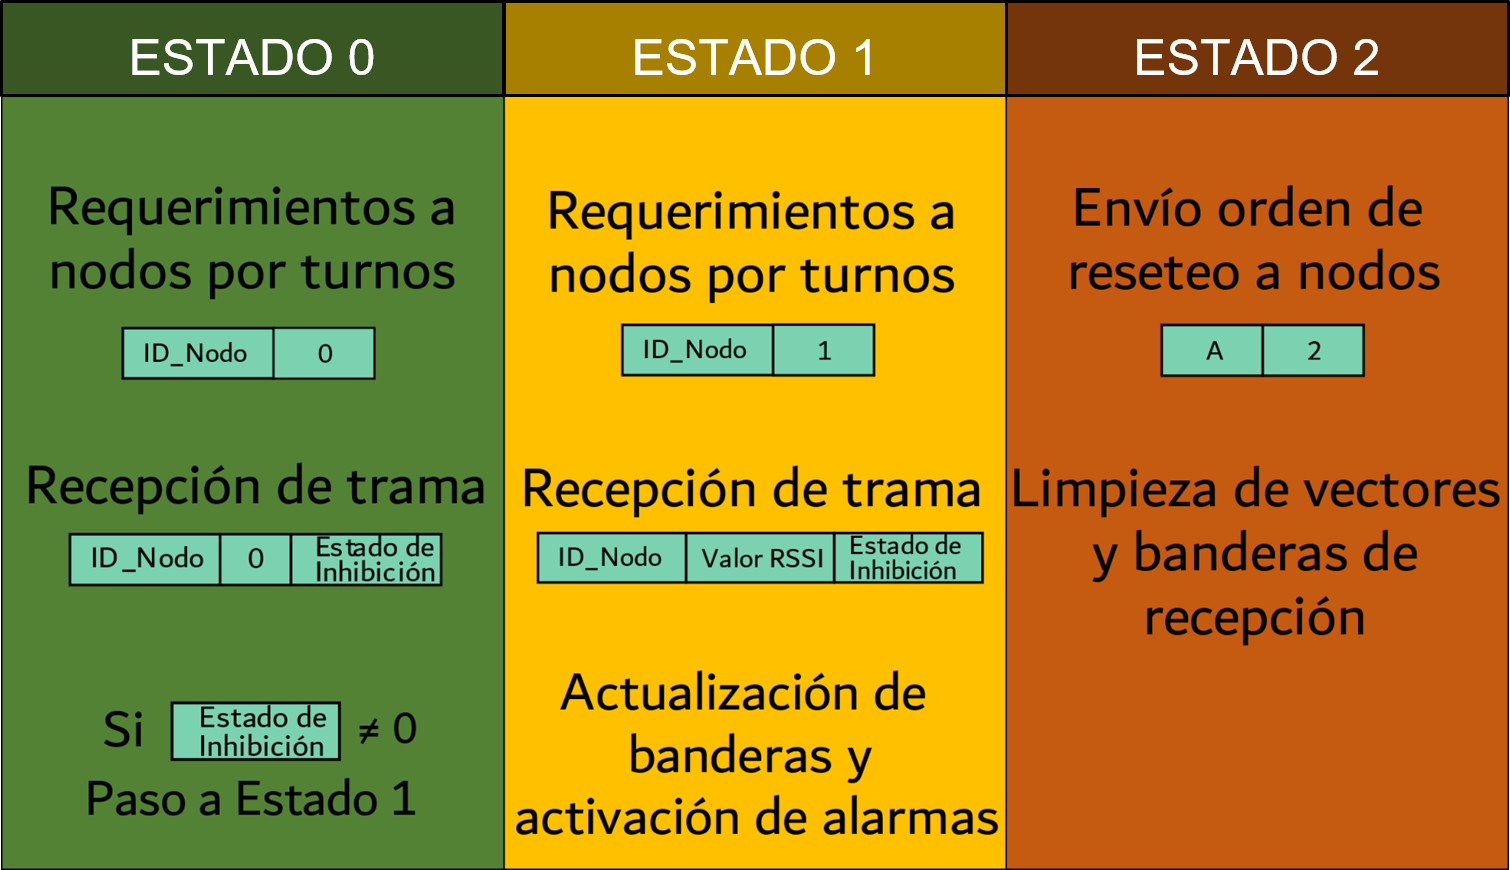
\includegraphics[scale=.53]{images/central/maquina-estado-central.png}
    \caption{Estados de la central en comunicación con nodos.}
	\label{im:maq-est-central}
\end{figure}


\subsubsection{Salud de nodos}
\par La salud de los nodos es un dato muy importante para saber que el sistema no falle, por ello la central tiene 3 leds en la parte frontal que indican si alguno no esta contestando los requerimientos pedidos, los cuales actualizan su estado en cada ciclo, permitiendo así una visualización en tiempo real de la misma. 

\subsubsection{Alarma sonora y visual}
\par Localmente, al haberse activado las alertas de inhibición presente se activa un indicador lumínico en la central y un pitido de 1 segundo para avisar al personal de seguridad o a la persona a cargo el hecho que ocurre. 

\subsubsection{Subida de datos al servidor web}
\par El enfoque que se le quiso dar a este sistema en general es la posibilidad de generar una base de datos de acceso remoto, no solo para poder triangular la posición en caso de ser posible, sino también pensando en que se pueda disponer este tipo de dispositivos en diferentes zonas y así generar estadísticas que tenga acceso cualquier persona y alertar sobre este tipo de episodios. 
\par El desenlace de carga de datos remotamente vía GPRS se da al fin del ciclo de detección. En este caso pasa algo particular, donde el integrado utilizado requiere que se le envíen una serie de comandos para ser ejecutados con cada acción y a su ves cada uno de ellos se puede enviar cada cierto tiempo. Por ello, para que el sistema no se congele cargando datos y dejando de escuchar los canales de 433.92MHz, esta se realiza en una interrupción del sistema, con los comandos a enviar cargados por DMA (direct memory access) y los retardos necesarios son generados por la cuenta de ticks (pulsos que se dan en el sistema cada 1ms) que no interrumpen la ejecución del código, permitiendo que mientras se cargan los datos, también se reinicie el sistema y se siga escuchando el canal por una nueva presencia de inhibición. 
\par La carga se realiza mediante un proceso de HTTP POST, que consiste de un formulario HTML, donde se le pasan los atributos necesarios para establecer el formato a cargar, en este caso se configura como "application/x-www-form-urlencoded", que indica que los datos se pasan en forma de tuplas llave-valor separadas por '\&' y un '=' entre la llave y el valor. Un ejemplo de como se vería la carga es:
\begin{lstlisting}
    POST / HTTP/1.1 
    Host: www.jammer-detector.ml
    Content-Type: application/x-www-form-urlencoded 
    Content-Length: 19
    
    RSSI=45&mode_inhi=1 
\end{lstlisting}
\subsection{Hardware}
\par En este apartado se mostrará una descripción de la placa que contiene el MCU, los esquemáticos finales, el pcb obtenido y su modelo en 3D. 


\subsubsection{Esquemático}
\par Como en el apartado de selección de componentes se ha explayado, como microcontrolador se hace uso del STM32F106C8T6. Este 
cuenta con un cristal de 8 MHz, el cual mediante un PLL interno es llevado a la frecuencia de operación de 72 MHz. En la
figura \ref{cristal_bluepill} se puede observar lo antes mencionado.

\begin{figure}[!h]
	\centering
	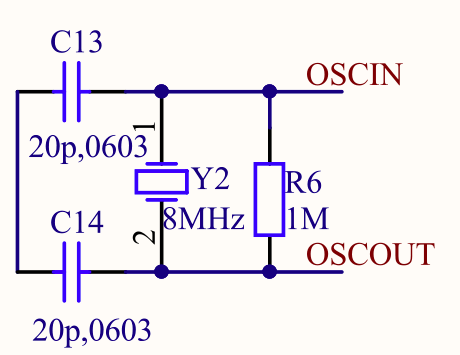
\includegraphics[scale=0.35]{images/central/bluepill-osc.png}
    \caption{Cristal para el MCU}
	\label{cristal_bluepill}
\end{figure}

\par También cuenta con un regulador de 5V a 3.3V (figura \ref{im:reg-bluepill}) para la alimentación a los pines que manejan estos niveles de lógica y es utilizado también para el debugger. Por último como se observa en la figura \ref{im:reset-bluepill}, la placa tiene un botón de reset el cual es activo por bajo. 

\begin{figure}[!h]
	\centering
	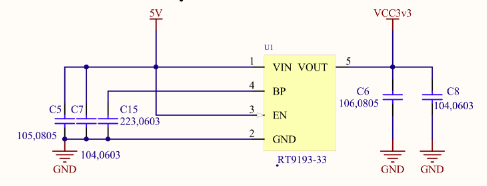
\includegraphics[scale=0.6]{images/central/bluepill-reg.png}
    \caption{Regulador de 5V a 3.3V para MCU.}
	\label{im:reg-bluepill}
\end{figure}

\begin{figure}[!h]
	\centering
	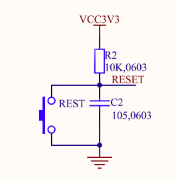
\includegraphics[scale=0.6]{images/central/bluepill-reset.png}
    \caption{Reset de microcontrolador.}
	\label{im:reset-bluepill}
\end{figure}

\par El esquemático en general se separó en varias partes para que se puedan observar de una manera mas ordenada en el presente informe. Estas 3 partes nombradas se pueden ver en las figuras \ref{im:esq-central-1}, \ref{im:esq-central-2} y \ref{im:esq-central-3} con su descripción de la correspondencia de cada una de ellas. 

\begin{figure}[!h]
	\centering
	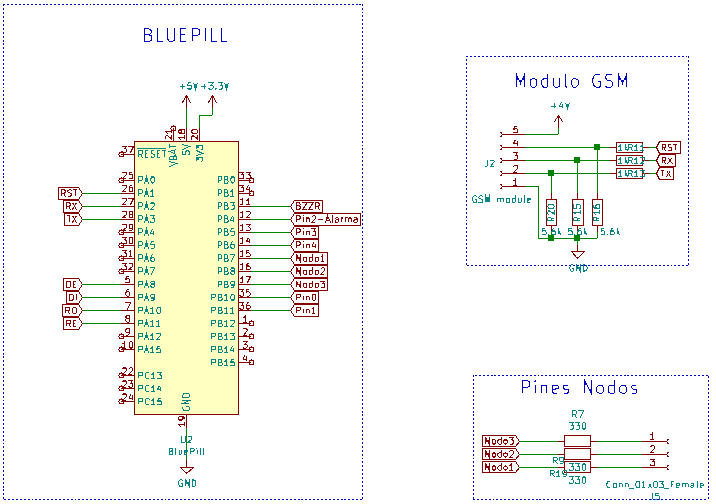
\includegraphics[scale=.50]{images/central/central-esq-1.png}
    \caption{MCU, modulo GSM/GPRS y leds indicadores de nodos.}
	\label{im:esq-central-1}
\end{figure}

\begin{figure}[!h]
	\centering
	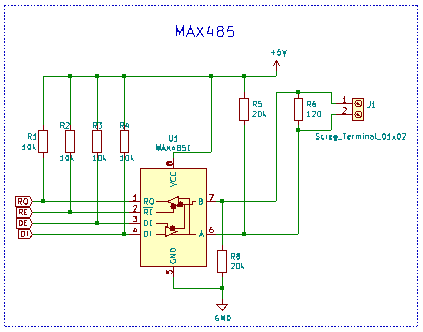
\includegraphics[scale=.59]{images/central/central-esq-2.png}
    \caption{Sección de comunicación RS485.}
	\label{im:esq-central-2}
\end{figure}

\begin{figure}[!h]
	\centering
	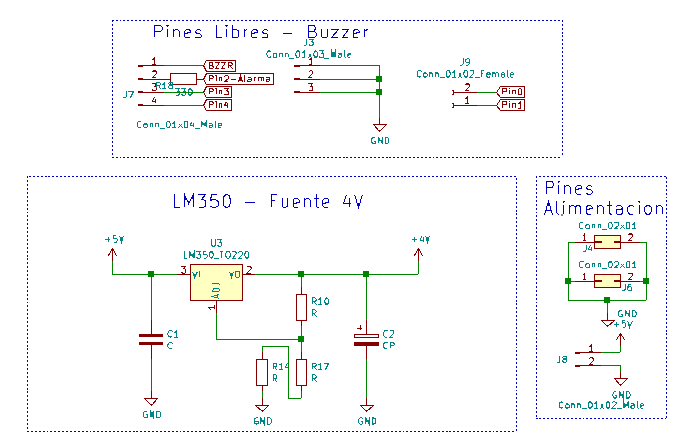
\includegraphics[scale=.55]{images/central/central-esq-3.png}
    \caption{Pines de alimentación, regulación para SIM800 y pines libres para conexiones adicionales.}
	\label{im:esq-central-3}
\end{figure}

\subsubsection{PCB}
En la figura \ref{im:pcb-final} vemos el diseño final de la placa de la central, el cual se diferencia al prototipo (figura \ref{im:pcb-prototipo}) en la fuente conmutada, que fue reemplazada por una lineal y en la adición de los leds indicadores de estado de cada nodo. 

\begin{figure}[!h]
\begin{center}
    \subfigure{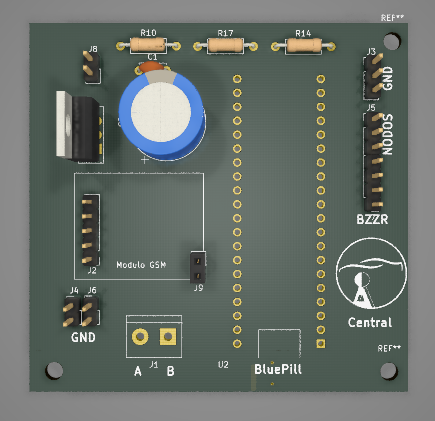
\includegraphics[width=60mm]{images/central/Central top.png}}
    \subfigure{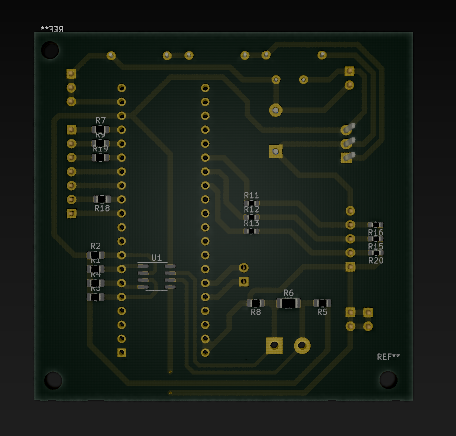
\includegraphics[width=60mm]{images/central/central-botton.png}}
    \caption{Diseño final de placa de la central de procesamiento.}
	\label{im:pcb-final}
\end{center}
\end{figure}

\subsubsection{Modelo 3D}
El modelo 3D de la placa la podemos observar en la figura \ref{im:mod-3d-central} y el resultado finalizado en la imagen \ref{placa_central}.

\begin{figure}[!h]
	\centering
	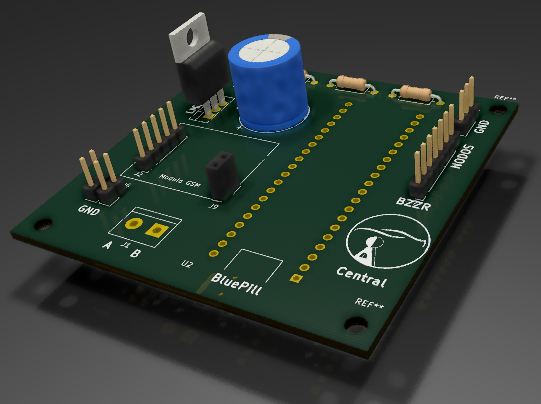
\includegraphics[scale=.55]{images/central/Central-perspectiva.png}
    \caption{Vista en 3D de la placa final de la central de procesamiento.}
	\label{im:mod-3d-central}
\end{figure}

\begin{figure}[!h]
	\centering
	\subfigure{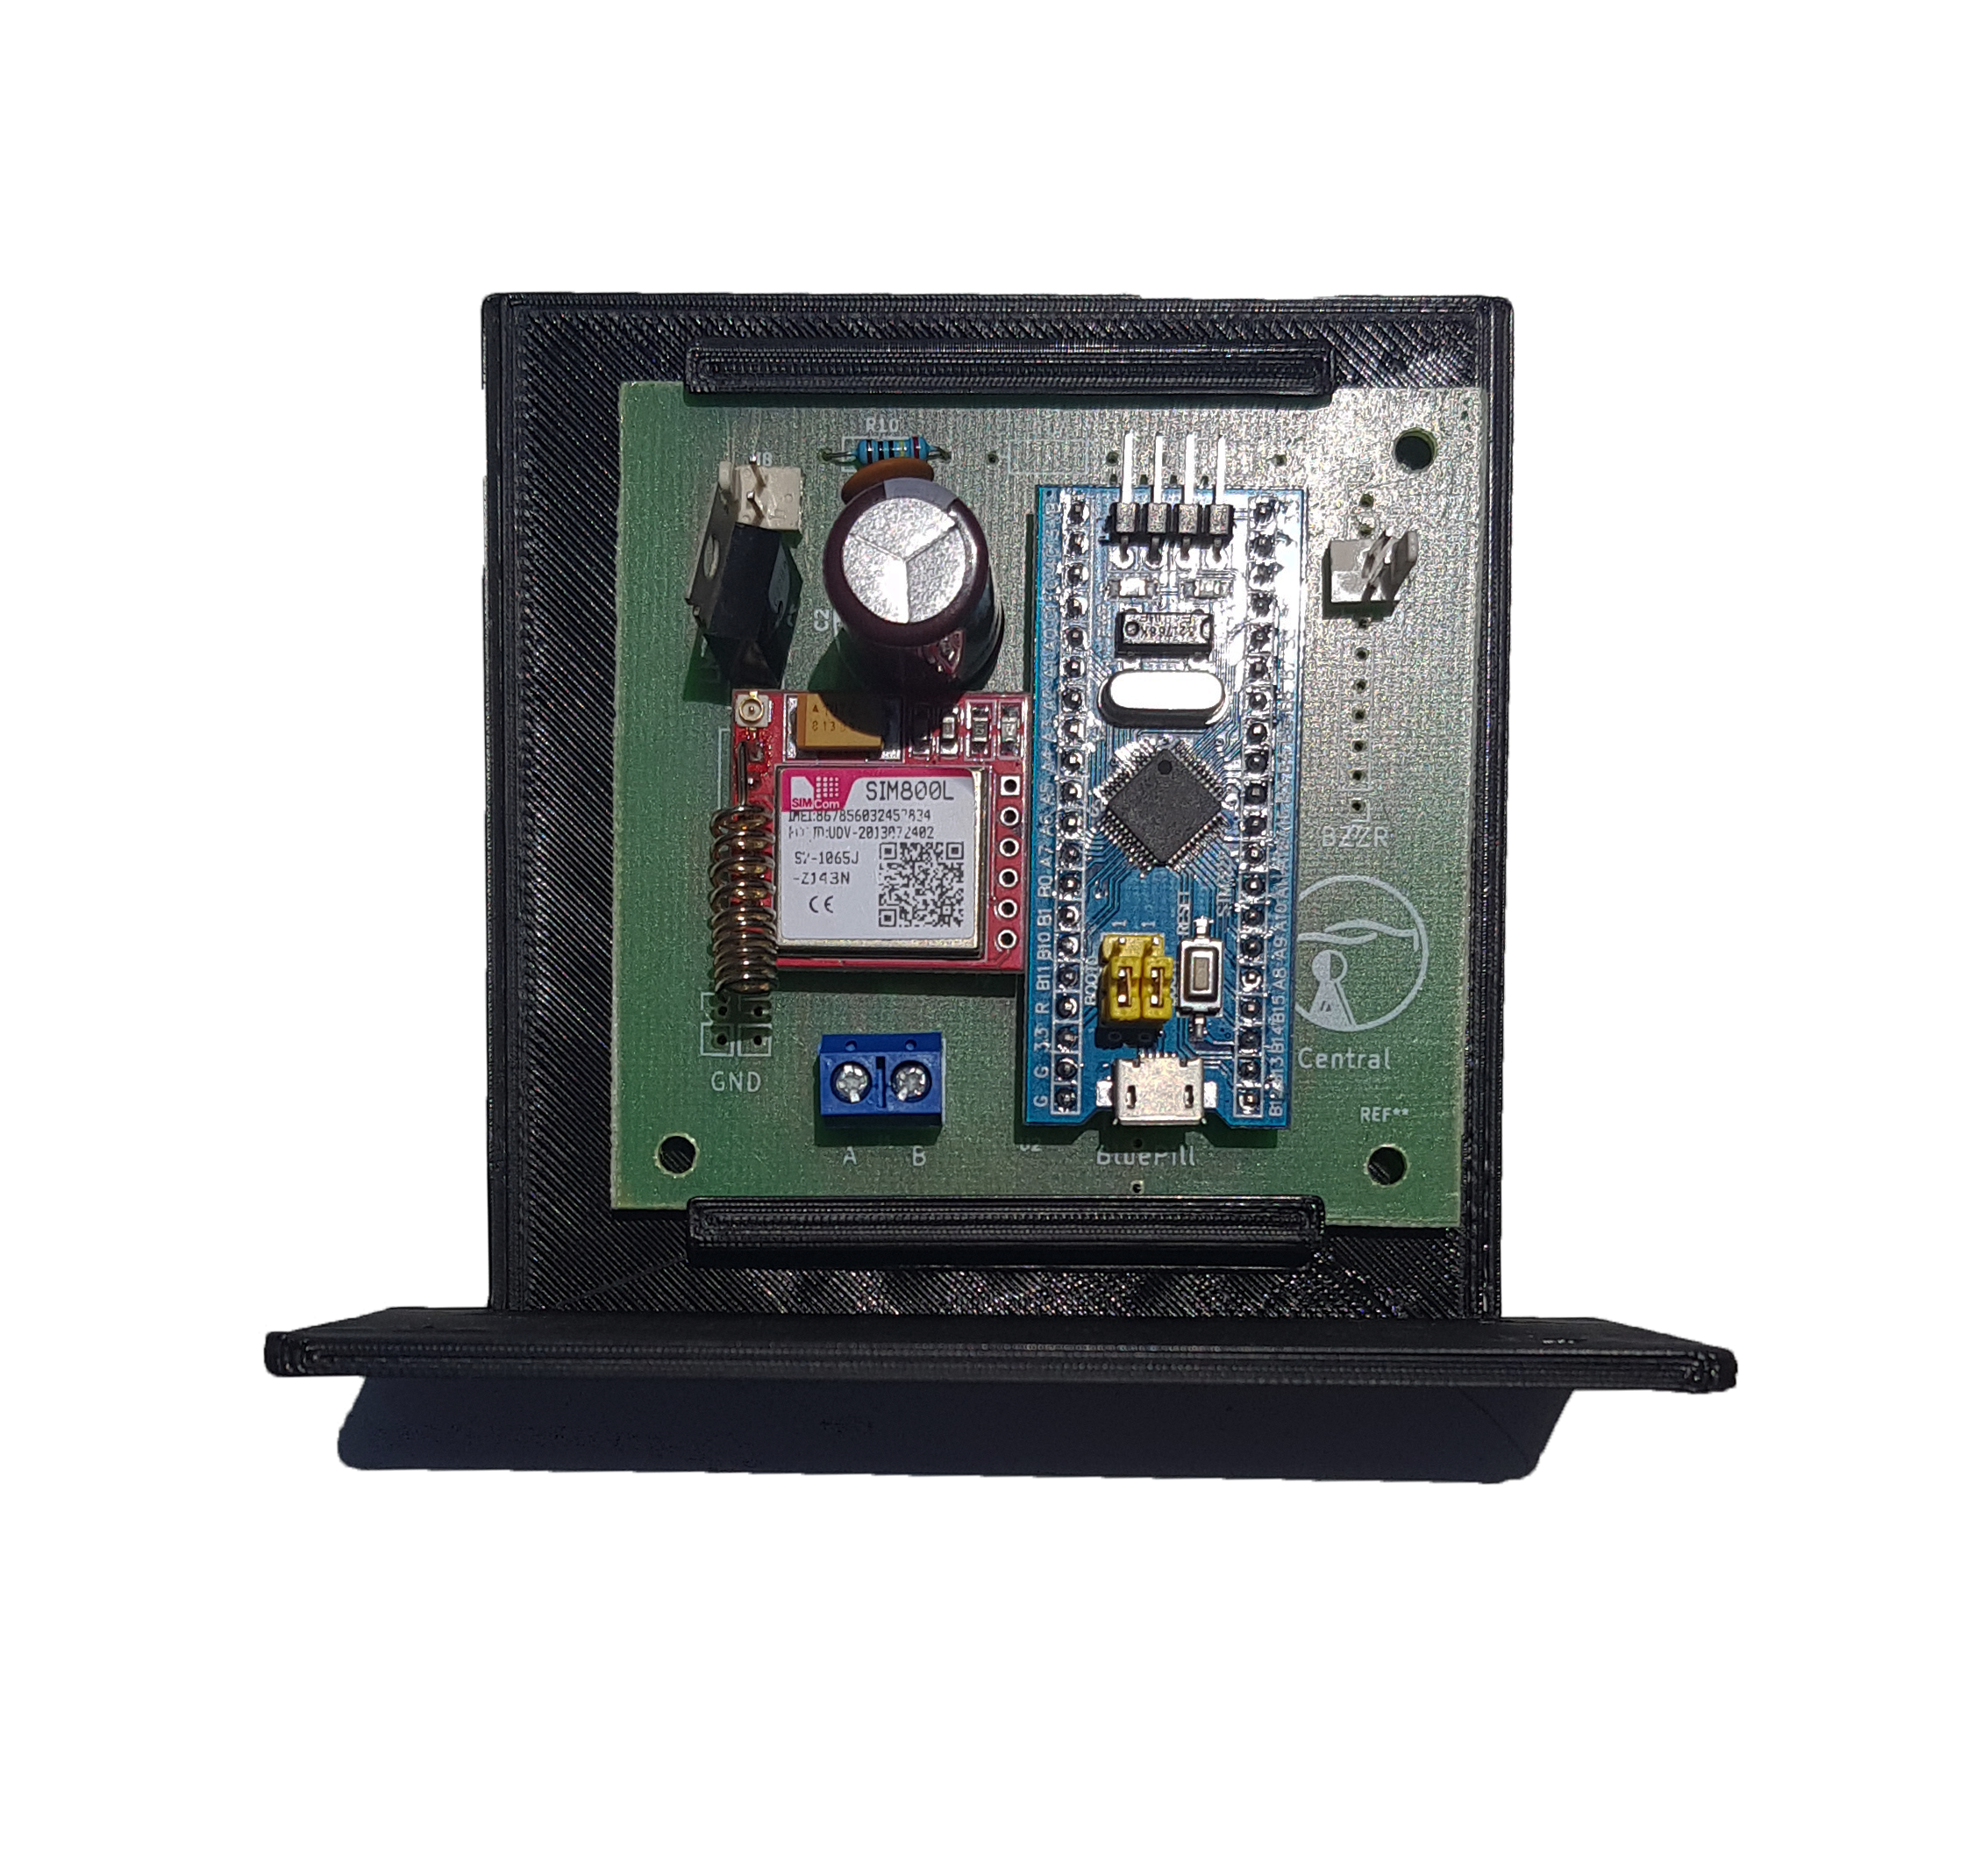
\includegraphics[width=105mm]{images/central/placa_central.png}}
    \caption{Placa de la central terminada.}
	\label{placa_central}
\end{figure}


\section{Gabinete}
\par El diseño del gabinete (figura \ref{im:gabinete-central}) de la central se busco que fuera de una forma vertical, en donde por delante se observen cinco indicadores lumínicos que informar sobre el estado de inhibición del sistema (agregado de un buzzer también), el estado de salud de cada nodo y si está en funcionamiento o no.
\par Por la parte trasera encontramos un interruptor para alimentar a todos los nodos, conector para 12V y un conector GXS para la comunicación RS485 y llevar la alimentación a cada nodo bajo el concepto de power over ethernet. 
\begin{figure}[!h]
\begin{center}
    \subfigure{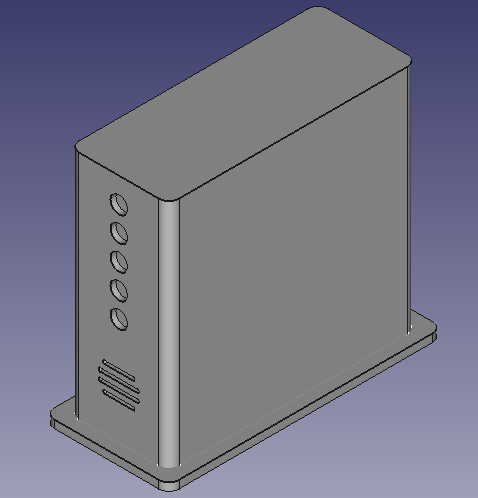
\includegraphics[width=55mm]{images/central/modelo-3d-central-frente.png}}
    \subfigure{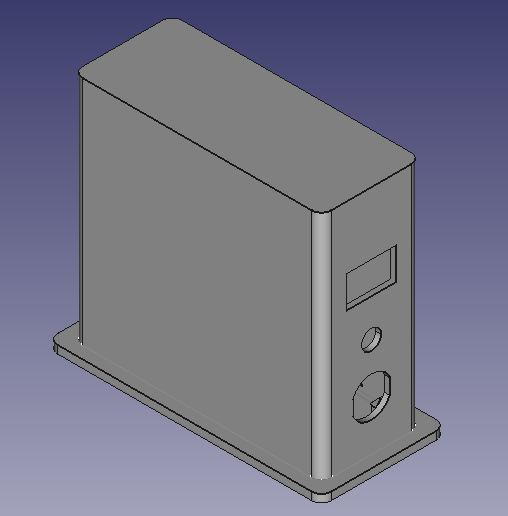
\includegraphics[width=56mm]{images/central/modelo-3d-central-atras.png}}
    \caption{Gabinete de central armado.}
	\label{im:gabinete-central}
\end{center}
\end{figure}

\par El mismo se llevo a la realidad por medio de impresión 3D en plástico PLA negro. Para comodidad en el armado e impresión, vemos en la figura \ref{im:impresion-central} que el modelo se dividió en 2 partes, donde una llamada "base" es la encargada de soportar la placa principal de la central y a la derecha de la imagen vemos lo 
que denominamos "tapa", donde encontramos los indicadores y demás conectores. 

\begin{figure}[!h]
	\centering
	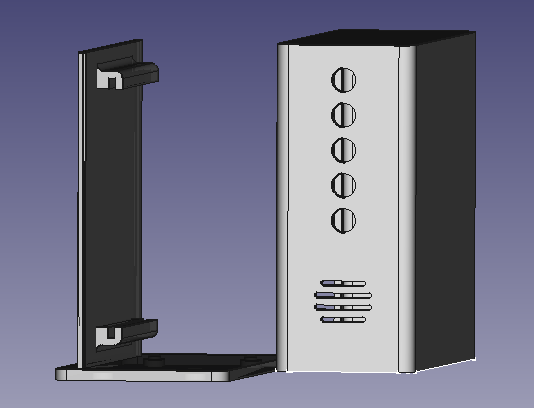
\includegraphics[scale=.53]{images/central/modelo-3d-central-separado.png}
    \caption{Partes para el armado del gabinete de central.}
	\label{im:impresion-central}
\end{figure}

En las figuras \ref{central} se puede apreciar el resultado final de la central en sus dos secciónes de impresión y con el gabinete
ya finalizado y ensamblado.

\begin{figure}[!h]
	\begin{center}
		\subfigure{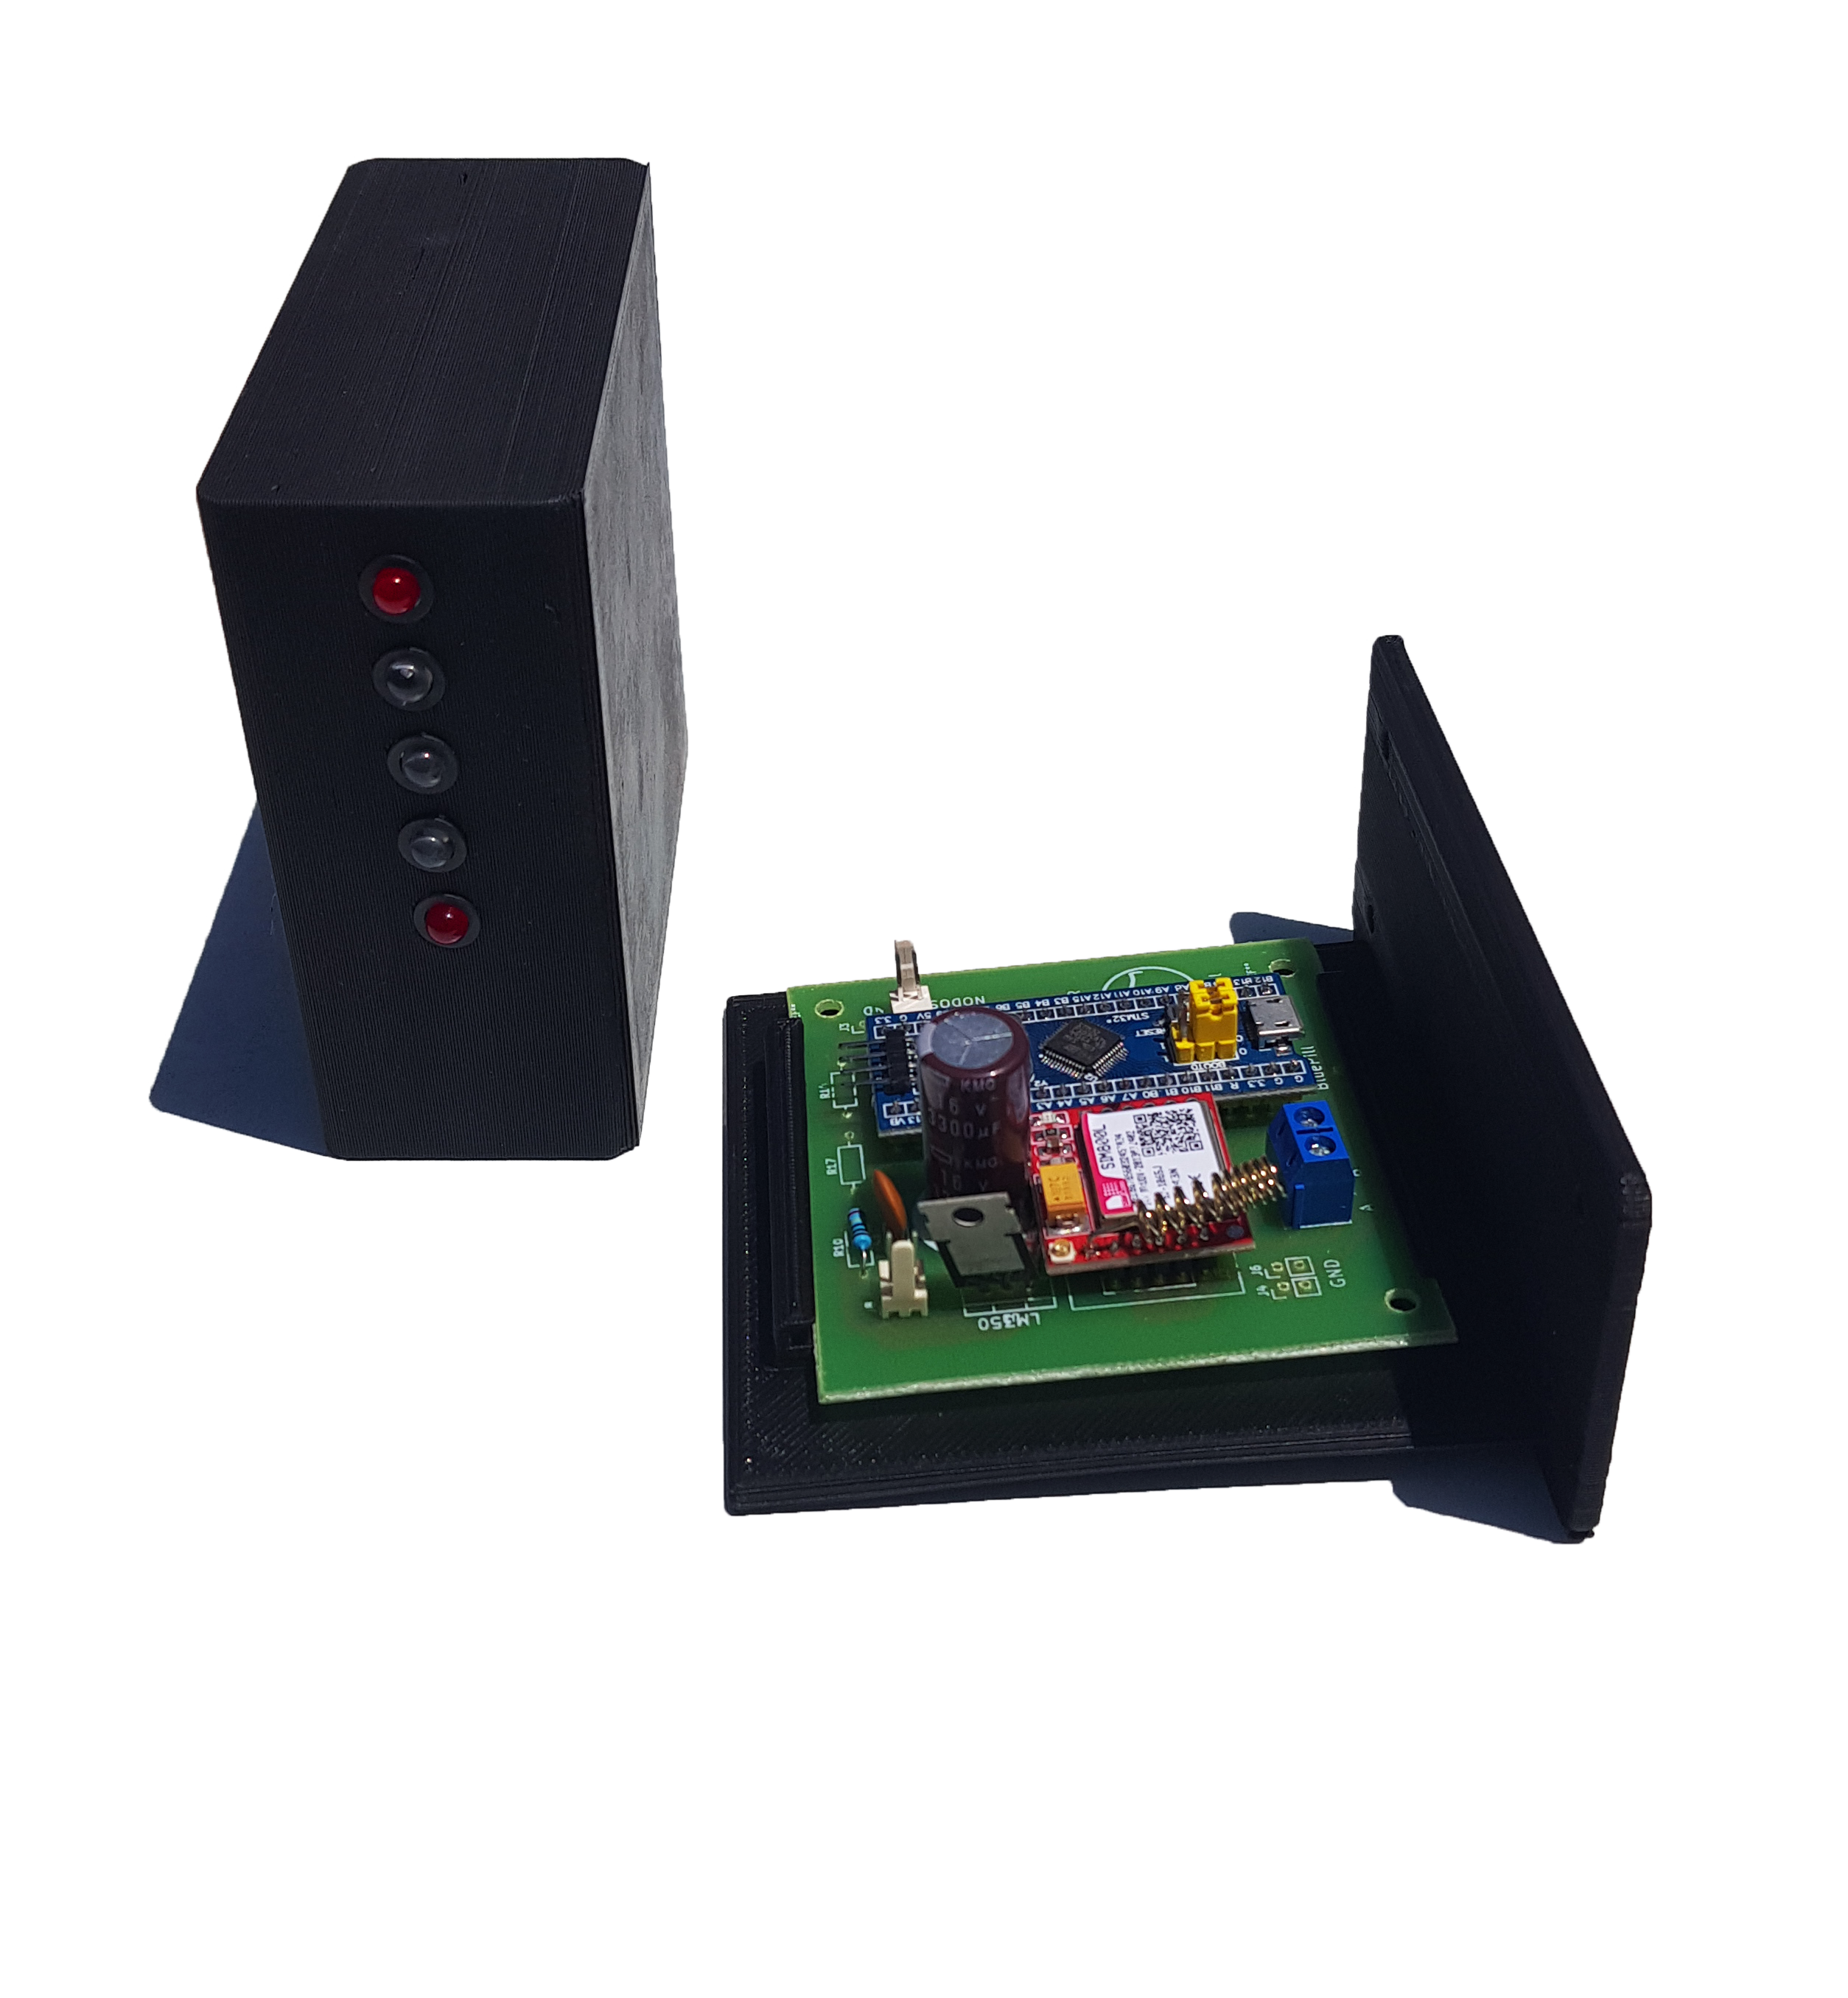
\includegraphics[width=75mm]{images/central/central_abierta.png}}
		\subfigure{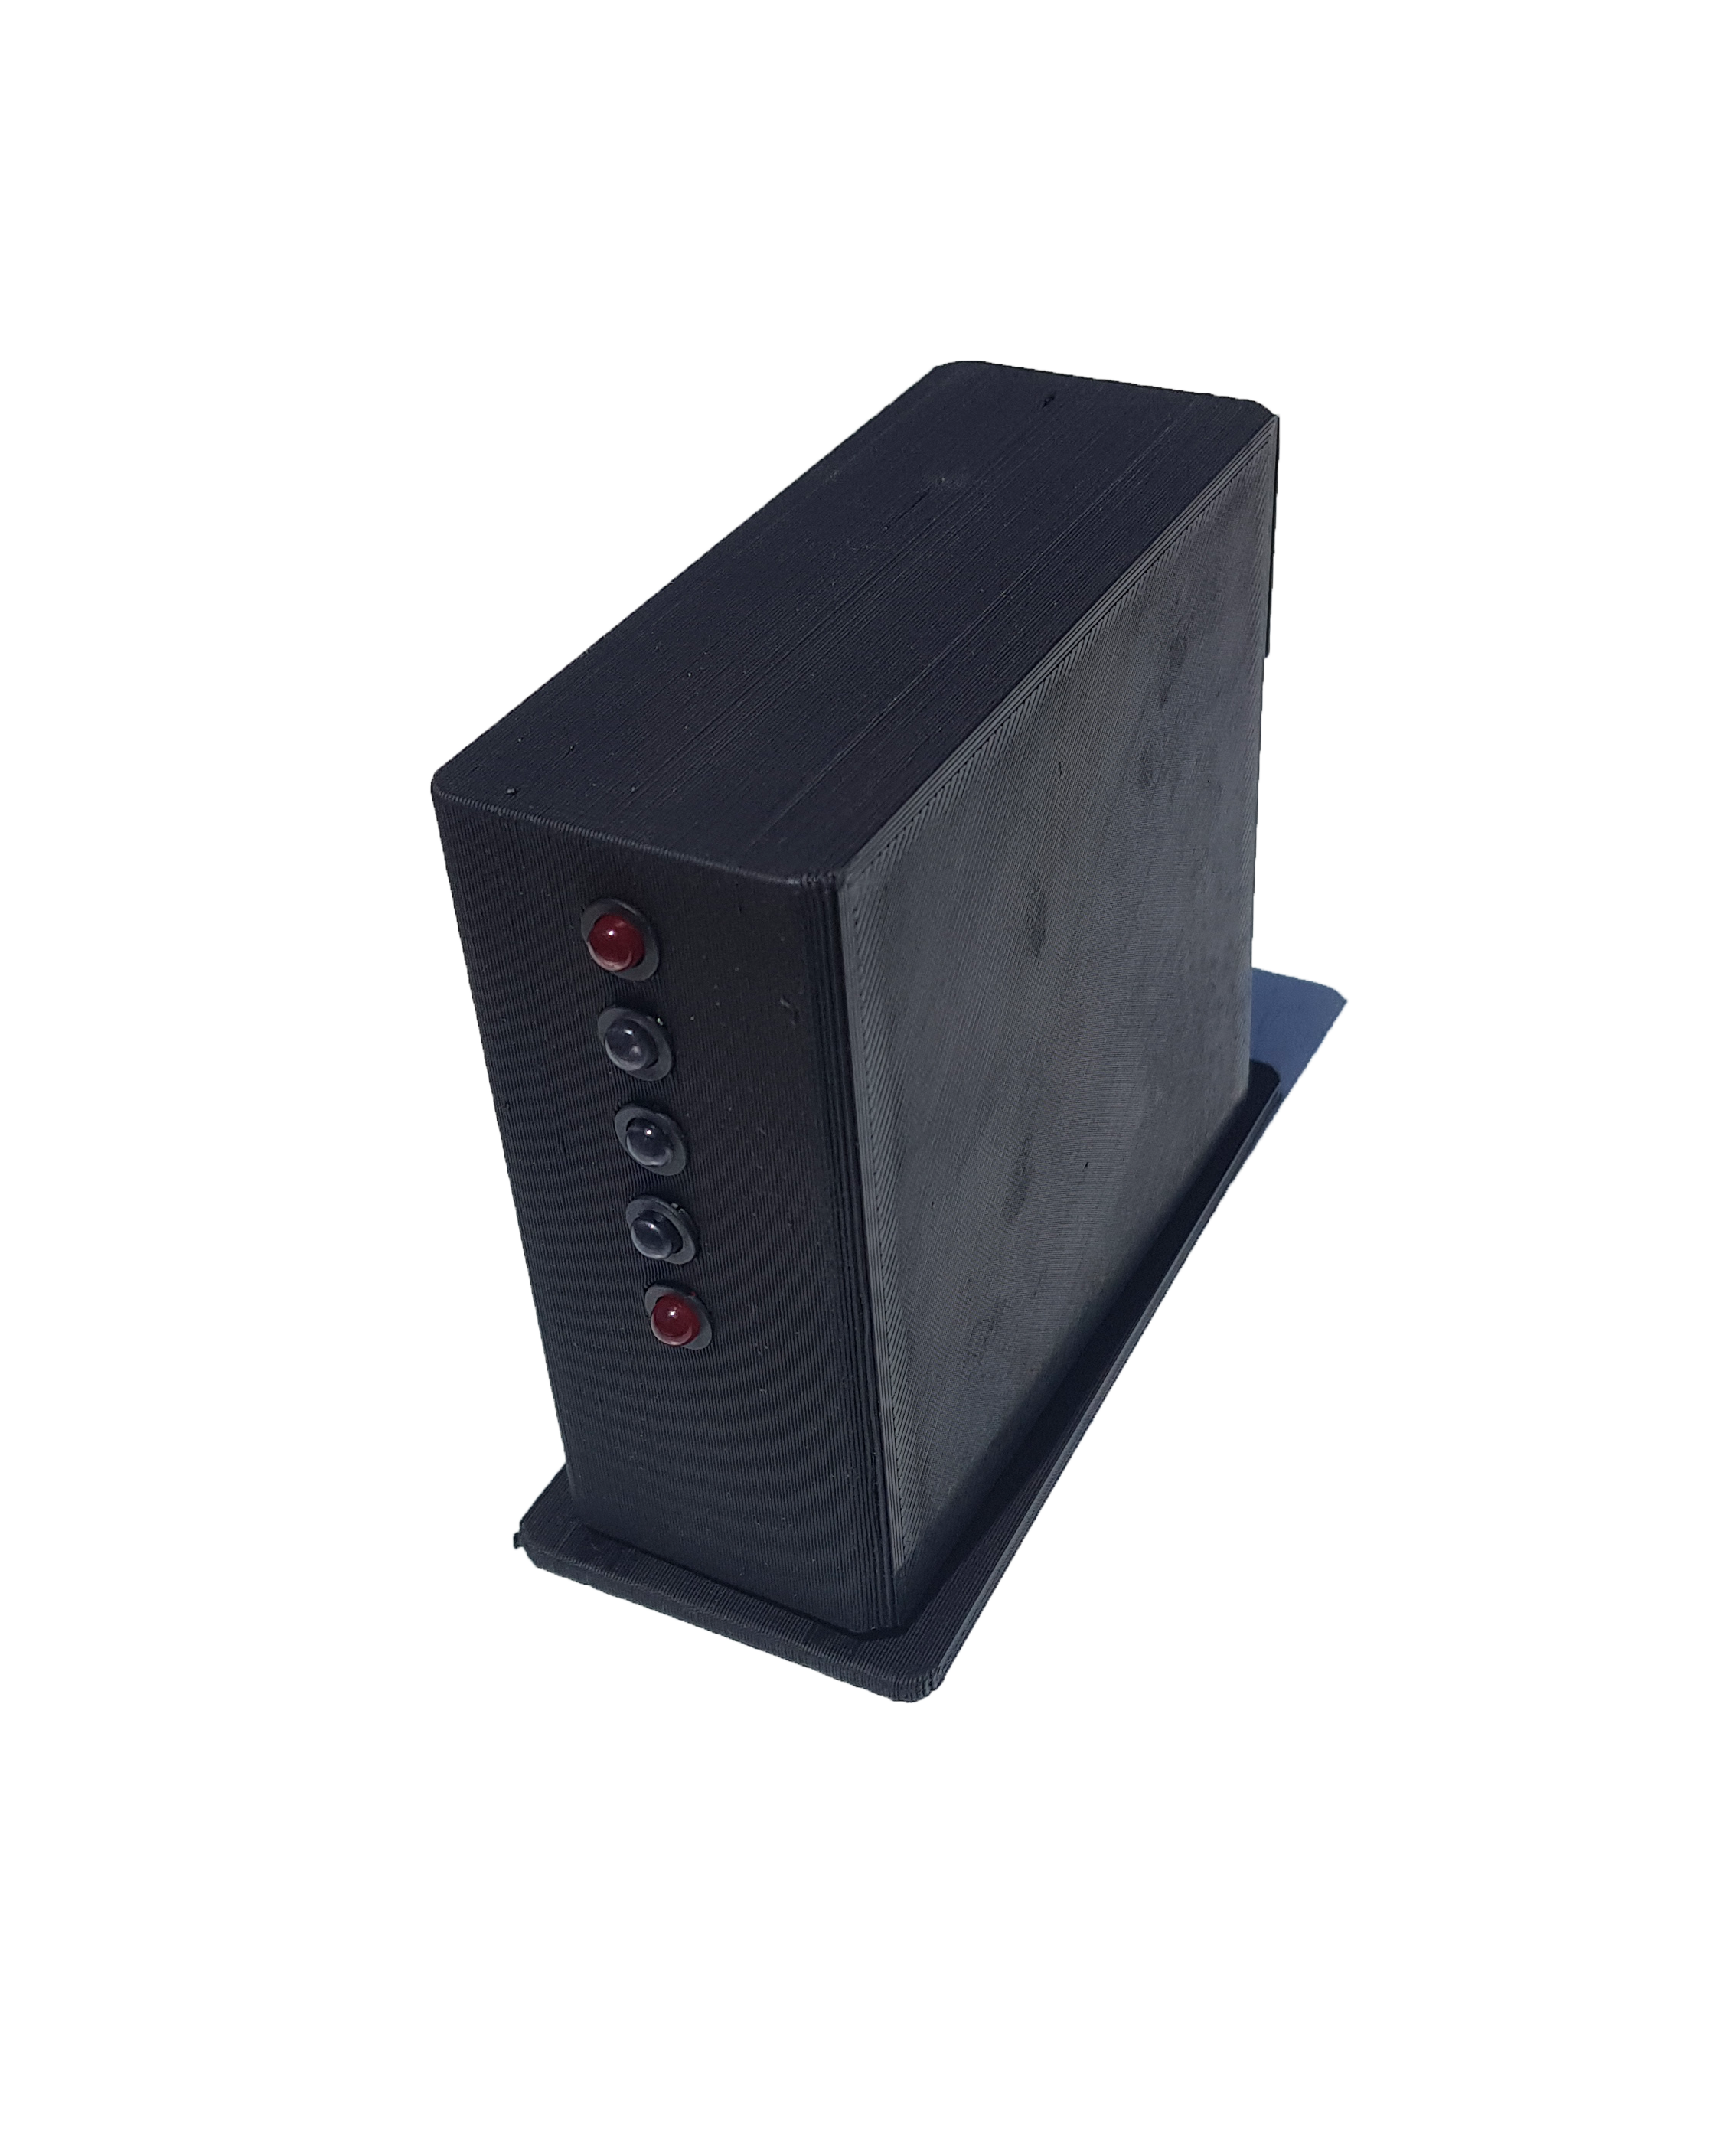
\includegraphics[width=76mm]{images/central/central_terminada.png}}
		\caption{Gabinete de central terminado.}
		\label{central}
	\end{center}
\end{figure}